
\documentclass[main.tex]{subfiles}

\begin{document}
\graphicspath{{imagenes/tema3/}{../imagenes/tema3/}}

% Diapositiva original 1
\portadatema{3}{Cálculo diferencial. Funciones de varias variables}
% Diapositiva original 2
\begin{frame}{Definición de derivada parcial}
Sea $z=f(x,y)$ una función de dos variables con dominio $D$. Si mantenemos fija la variable $y=b$, siendo $b$ constante, y suponemos que sólo varía $x$, $f$ se convierte en una función de una variable: $g(x)=f(x,b)$.
\medskip

Si $g$ tiene derivada en $a$, ésta se llama derivada parcial de $f$ respecto de $x$ en $(a,b)$, y se denota por $f_x(a,b)$.
\[f_x(a,b)=g'(a)=\lim_{h\to0}\frac{g(a+h)-g(a)}h.\]
\[f_x(a,b)=\lim_{h\to0}\frac{f(a+h,b)-f(a,b)}h.\]
\end{frame}
% Diapositiva original 3
\begin{frame}{Definición de derivada parcial}
Análogamente, sea $z=f(x,y)$ una función de dos variables. Si mantenemos fija la variable $x=a$, siendo $a$ constante, y suponemos que sólo varía $y$, $f$ se convierte en una función de una variable: $h(y)=f(a,y)$.
\medskip

Si $h$ tiene derivada en $b$, ésta se llama derivada parcial de $f$ respecto de $y$ en $(a,b)$, y se denota por $f_y(a,b)$.
\medskip

Por definición,
\[f_y(a,b)=\lim_{k\to0}\frac{f(a,b+k)-f(a,b)}k.\]
\end{frame}
% Diapositiva original 4
\begin{frame}{Derivadas parciales. Notación}
Dada una función de dos variables $z=f(x,y)$, otra notación para la derivada parcial de $f$ respecto de las variables $x$ e $y$ es
\[f_x=z_x=\frac{\partial f}{\partial x},\qquad f_y=z_y=\frac{\partial f}{\partial y}.\]
\end{frame}
% Diapositiva original 5
\begin{frame}{Derivadas parciales}
\textbf{Ejemplo}\par Calcular las derivadas parciales de\[f(x,y)=3x^2+xy^3+y\]
en el punto $(1,1)$.
\end{frame}
% Diapositiva original 6
\begin{frame}{Derivadas parciales}
\textbf{Ejemplo}\[f(x,y)=3x^2+xy^3+y\]
\[\begin{aligned}
\frac{\partial f}{\partial x}&=6x+y^3,&\frac{\partial f}{\partial x}(1,1)&=7,\\[3mm]
\frac{\partial f}{\partial y}&=3xy^2+1,&\frac{\partial f}{\partial y}(1,1)&=4.
\end{aligned}\]
\end{frame}
% Diapositiva original 7
\begin{frame}{Derivadas parciales}
\textbf{Ejercicio}\par Calcular las derivadas parciales de\[f(x,y)=e^x\ln(xy).\]
\end{frame}
% Diapositiva original 8
\begin{frame}{Interpretación geométrica}
\small Si consideramos la superficie $z=f(x,y)$, el plano $y=b$ la corta en la curva $z=f(x,b)$. La pendiente de esta curva en $x=a$ es la derivada parcial respecto de $x$, $f_x(a,b)$.
\begin{columns}[c]\begin{column}{.48\textwidth}\figura{corte_x_3d.png}{1}{.57}\end{column}\begin{column}{.48\textwidth}\figura{corte_x_2d.png}{1}{.57}\end{column}\end{columns}
\end{frame}
% Diapositiva original 9
\begin{frame}{Interpretación geométrica}
\small Análogamente, al cortar la superficie por el plano $x=a$ se obtiene la curva $z=f(a,y)$. La pendiente de esta curva en $y=b$ es la derivada parcial respecto de $y$, $f_y(a,b)$.
\begin{columns}[c]\begin{column}{.48\textwidth}\figura{corte_y_3d.png}{1}{.57}\end{column}\begin{column}{.48\textwidth}\figura{corte_y_2d.png}{1}{.57}\end{column}\end{columns}
\end{frame}
% Diapositiva original 10
\begin{frame}{Interpretación geométrica}
\figura{cortes.png}{.95}{.82}
\end{frame}
% Diapositiva original 11
\begin{frame}{Plano tangente}
\small En una variable, la existencia de una derivada finita en un punto equivale a la existencia de la recta tangente no vertical en ese punto.
\medskip

Para dos variables, la diferenciabilidad en $(a,b)$ permite aproximar la superficie por su plano tangente en $(a,b,f(a,b))$.
\medskip

\textbf{Teorema}\par Si $f$ es diferenciable en $(a,b)$, la ecuación del plano tangente es
\[f_x(a,b)(x-a)+f_y(a,b)(y-b)-(z-f(a,b))=0.\]
\end{frame}
% Diapositiva original 12
\begin{frame}{Plano tangente}
\figura{plano_tangente.png}{.95}{.83}
\end{frame}
% Diapositiva original 13
\begin{frame}{Plano tangente}
\textbf{Ejercicio}\par Calcular el plano tangente a\[f(x,y)=3x^2+xy^3+y\]
en el punto $(1,1)$.
\end{frame}
% Diapositiva original 14
\begin{frame}{Derivadas de funciones paramétricas}
\small Tenemos dos formas de realizarlas. Lo veremos con un ejemplo.
\medskip

Sea $f(x,y)=xy^2-x^2$, con $x=\cos t$, $y=\sin t$. Calcular la derivada respecto a $t$.
\medskip

\textbf{1)} Sustituimos $x$ e $y$ en $f$ y derivamos respecto a $t$:
\[f(t)=\cos t\,\sin^2t-\cos^2t.\]
\[f'(t)=-\sin^3t+2\cos^2t\sin t+2\sin t\cos t.\]
\end{frame}
% Diapositiva original 15
\begin{frame}{Regla de la cadena}
\small\textbf{Ejercicio}\par Sea $z=f(x,y)=xy^2-x^2$, con $x=\cos t$, $y=\sin t$. Calcular la derivada de $z$ respecto a $t$.
\medskip

\textbf{2)} Aplicamos la regla de la cadena:
\[f'(t)=f_xx'(t)+f_yy'(t).\]
\[f'(t)=(y^2-2x)(-\sin t)+2xy\cos t.\]
\[=(\sin^2t-2\cos t)(-\sin t)+2\cos^2t\sin t.\]
\figura{cadena_t.png}{.38}{.24}
\end{frame}
% Diapositiva original 16
\begin{frame}{Regla de la cadena}
\small Tenemos una función de dos variables $z=f(x,y)$ y, a su vez, cada variable depende de dos parámetros: $x=g(u,v)$, $y=h(u,v)$. Las derivadas parciales serán
\[f_u=z_u=z_xx_u+z_yy_u,\qquad f_v=z_v=z_xx_v+z_yy_v.\]
\figura{cadena_uv.png}{.65}{.49}
\end{frame}
% Diapositiva original 17
\begin{frame}{Regla de la cadena}
\textbf{Ejercicio}\par Sea
\[z=f(x,y)=\frac{x^2y^2}{2},\qquad x=u+v,\quad y=u-v.\]
Calcular $f_u$ y $f_v$ de dos formas distintas: sustituyendo $x$ e $y$, y aplicando el teorema anterior.
\end{frame}
% Diapositiva original 18
\begin{frame}{Derivación implícita}
\textbf{Ejemplo}\par Sabiendo que $z=f(x,y)$, calcular $z_x$ y $z_y$ de la ecuación implícita
\[z^3\sin x+ze^{xy}-xy=0.\]
\end{frame}
% Diapositiva original 19
\begin{frame}{Funciones de varias variables}
\small\textbf{Derivadas parciales de funciones de tres variables}\par Para $f(x,y,z)$, se definen
\[f_x=\frac{\partial f}{\partial x},\qquad f_y=\frac{\partial f}{\partial y},\qquad f_z=\frac{\partial f}{\partial z}\]
como las derivadas respecto de $x$, $y$ o $z$, dejando las otras dos variables constantes.
\medskip

\textbf{Para funciones de $n$ variables}\par $f:\mathbb R^n\to\mathbb R$, $f(x_1,\ldots,x_n)$:
\[f_{x_j}=\frac{\partial f}{\partial x_j},\quad j=1,\ldots,n.\]
Para $\mathbf x=(x_1,\ldots,x_n)$ y el vector $\mathbf e_j$ con componente $j$ igual a 1 y las demás iguales a 0,
\[\frac{\partial f}{\partial x_j}(\mathbf x)=\lim_{\lambda\to0}\frac{f(\mathbf x+\lambda\mathbf e_j)-f(\mathbf x)}{\lambda}.\]
\end{frame}
% Diapositiva original 20
\begin{frame}{Vector gradiente}
\small Se define el \textbf{vector gradiente} de una función de $n$ variables como el vector cuyas componentes son las derivadas parciales.
\[\nabla f=(f_{x_1},\ldots,f_{x_n})=\left(\frac{\partial f}{\partial x_1},\ldots,\frac{\partial f}{\partial x_n}\right)\]
La derivada de una función real de variable real informa de su tasa de variación por unidad de cambio de la variable independiente en un punto.
\medskip

Cada componente del gradiente informa de la tasa de variación de la función respecto de una variable, manteniendo las demás constantes.
\end{frame}
% Diapositiva original 21
\begin{frame}{Vector gradiente}
\small\[\nabla f=(f_{x_1},\ldots,f_{x_n})=\left(\frac{\partial f}{\partial x_1},\ldots,\frac{\partial f}{\partial x_n}\right)\]
Como cada derivada parcial en un punto es un número real, el gradiente es un conjunto ordenado de números reales: un vector cuya dimensión es el número de variables.
\medskip

Para una función de tres variables,
\[\nabla f(x,y,z)=(f_x,f_y,f_z)=f_x\mathbf i+f_y\mathbf j+f_z\mathbf k.\]
\end{frame}
% Diapositiva original 22
\begin{frame}{Vector gradiente}
\small\textbf{Ejemplo}\par Calcular el gradiente de la función de tres variables
\[f(x,y,z)=3x^2yz+5xz+6\]
\[\nabla f=(6xyz+5z,\,3x^2z,\,3x^2y+5x)\]
\[=(6xyz+5z)\mathbf i+3x^2z\mathbf j+(3x^2y+5x)\mathbf k.\]
El gradiente en los puntos $(0,2,-1)$ y $(1,-1,-1)$ vale
\[\nabla f(0,2,-1)=(-5,0,0)=-5\mathbf i,\]
\[\nabla f(1,-1,-1)=(1,-3,2)=\mathbf i-3\mathbf j+2\mathbf k.\]
\end{frame}
% Diapositiva original 23
\begin{frame}{Propiedades del gradiente}
\small El vector gradiente de una función diferenciable, si es no nulo, señala la dirección de máximo crecimiento de la función en el punto considerado. Entre todas las direcciones, la definida por el gradiente es aquella en la que la función crece más rápidamente.
\medskip

La dirección opuesta al gradiente es aquella en la que la función decrece más rápidamente.
\medskip

$\nabla f(x,y)$ es un vector en el plano y $\nabla f(x,y,z)$ es un vector en el espacio. Si el gradiente es cero, todas las derivadas direccionales son cero.
\end{frame}
% Diapositiva original 24
\begin{frame}{Propiedades del gradiente}
Esta propiedad tiene importancia en muchas situaciones reales. Por ejemplo, en la quimiotaxis, algunas células se mueven de acuerdo con la concentración de ciertas sustancias químicas en su medio ambiente.
\medskip

Pueden elegir la dirección del gradiente de la concentración para buscar alimento, o la opuesta al gradiente para alejarse de un veneno.
\end{frame}
% Diapositiva original 25
\begin{frame}{Vector gradiente}
\begin{columns}[c]
\begin{column}{.59\textwidth}\figura{gradiente.png}{1}{.65}\[\nabla f(x,y)\]\end{column}
\begin{column}{.39\textwidth}El gradiente no nulo es perpendicular a la curva de nivel de $f$ que pasa por el punto $(x_0,y_0)$.\end{column}
\end{columns}
\end{frame}
% Diapositiva original 26
\begin{frame}{Vector gradiente}
\small\textbf{Ejemplo}\par La temperatura, en grados Celsius, en la superficie de una placa metálica es
\[T(x,y)=20-4x^2-y^2.\]
$x$ e $y$ se miden en centímetros. ¿En qué dirección, a partir de $(2,-3)$, aumenta más rápido la temperatura? ¿Cuál es la tasa de crecimiento?
\[\nabla T(x,y)=-8x\mathbf i-2y\mathbf j,\quad\nabla T(2,-3)=-16\mathbf i+6\mathbf j.\]
Ésta es la dirección de máximo crecimiento. La dirección unitaria es $(-16,6)/\sqrt{292}$ y la tasa máxima es
\[\|\nabla T(2,-3)\|=\sqrt{256+36}=\sqrt{292}\approx17{,}09\ ^\circ\mathrm C/\mathrm{cm}.\]
\end{frame}
% Diapositiva original 27
\begin{frame}{Derivada direccional}
La derivada direccional es el producto escalar del gradiente por el vector unitario que determina la dirección.
\medskip

Si $f$ es diferenciable, su derivada direccional en la dirección del vector unitario $\mathbf u$ es
\[D_{\mathbf u}f(x,y)=\nabla f(x,y)\cdot\mathbf u.\]
\end{frame}
% Diapositiva original 28
\begin{frame}{Derivada direccional}
El concepto de derivada direccional se puede explicar con el siguiente ejemplo.
\medskip

Supongamos que nos encontramos sobre una superficie inclinada, por ejemplo, en la ladera de una montaña. Dependiendo de la dirección en que caminemos, descenderemos o ascenderemos y encontraremos una mayor o menor pendiente.
\end{frame}
% Diapositiva original 29
\begin{frame}{Derivada direccional}
\textbf{Ejemplo}\par Obtener la derivada direccional de\[f(x,y,z)=3x^2yz+5xz+6\]
en la dirección del vector $(1,-2,-1)$.
\end{frame}
% Diapositiva original 30
\begin{frame}{Derivada direccional}
\small\textbf{Ejemplo}\[f(x,y,z)=3x^2yz+5xz+6\]
En la dirección del vector $(1,-2,-1)$:
\[\nabla f=(6xyz+5z,\,3x^2z,\,3x^2y+5x)\]
El vector tiene módulo $\sqrt6$, por lo que $\mathbf u=(1,-2,-1)/\sqrt6$.
\[D_{\mathbf u}f=(6xyz+5z,3x^2z,3x^2y+5x)\cdot\left(\frac1{\sqrt6},\frac{-2}{\sqrt6},\frac{-1}{\sqrt6}\right).\]
\[D_{\mathbf u}f=\sqrt6xyz+\frac5{\sqrt6}z-\sqrt6x^2z-\sqrt{\frac32}x^2y-\frac5{\sqrt6}x.\]
\end{frame}
% Diapositiva original 31
\begin{frame}{Matriz jacobiana}
\small Dado un conjunto de funciones $\mathbf f=(f_1,\ldots,f_s)$, de $q$ variables cada una, la matriz jacobiana $J_{\mathbf f}$ tiene $s$ filas y $q$ columnas. Su elemento en la fila $i$, columna $j$, es $\partial f_i/\partial x_j$.
\[J_{\mathbf f}=\begin{pmatrix}
\frac{\partial f_1}{\partial x_1}&\frac{\partial f_1}{\partial x_2}&\cdots&\frac{\partial f_1}{\partial x_q}\\
\frac{\partial f_2}{\partial x_1}&\frac{\partial f_2}{\partial x_2}&\cdots&\frac{\partial f_2}{\partial x_q}\\
\vdots&\vdots&\ddots&\vdots\\
\frac{\partial f_s}{\partial x_1}&\frac{\partial f_s}{\partial x_2}&\cdots&\frac{\partial f_s}{\partial x_q}
\end{pmatrix}.\]
\end{frame}
% Diapositiva original 32
\begin{frame}{Matriz jacobiana}
\textbf{Ejemplo}\par Hallar la matriz jacobiana en $\mathbf a=(1,1,1)$ de la función\[f(x,y,z)=e^{x+y^3+z^2}.\]
\end{frame}
% Diapositiva original 33
\begin{frame}{Matriz jacobiana}
\small\textbf{Ejemplo}\par Hallar la matriz jacobiana en $\mathbf a=(1,1,1)$ de
\[f(x,y,z)=e^{x+y^3+z^2}.\]
\[f_x=e^{x+y^3+z^2},\quad f_y=3y^2e^{x+y^3+z^2},\quad f_z=2ze^{x+y^3+z^2}.\]
\[f_x(1,1,1)=e^3,\quad f_y(1,1,1)=3e^3,\quad f_z(1,1,1)=2e^3.\]
\[J_f(x,y,z)=\begin{pmatrix}e^{x+y^3+z^2}&3y^2e^{x+y^3+z^2}&2ze^{x+y^3+z^2}\end{pmatrix}.\]
\[J_f(1,1,1)=\begin{pmatrix}e^3&3e^3&2e^3\end{pmatrix}.\]
\end{frame}
% Diapositiva original 34
\begin{frame}{Matriz jacobiana}
\textbf{Ejercicio}\par Hallar la matriz jacobiana de
\[F=(f_1,f_2,f_3)=\bigl(x^2y^3,e^{x^2+y^4},\sin(2\pi y)\bigr).\]
\end{frame}
% Diapositiva original 35
\begin{frame}{Derivadas parciales segundas}
\small Se obtienen derivando parcialmente respecto de una variable $x_i$, dejando las demás fijas, y volviendo a derivar el resultado respecto de otra variable $x_j$ o de la misma variable $x_i$.
\[f_{xx}=\frac{\partial}{\partial x}\left(\frac{\partial f}{\partial x}\right)=\frac{\partial^2f}{\partial x^2},\quad
f_{yy}=\frac{\partial}{\partial y}\left(\frac{\partial f}{\partial y}\right)=\frac{\partial^2f}{\partial y^2}.\]
\[f_{xy}=\frac{\partial}{\partial y}\left(\frac{\partial f}{\partial x}\right)=\frac{\partial^2f}{\partial y\partial x},\quad
f_{yx}=\frac{\partial}{\partial x}\left(\frac{\partial f}{\partial y}\right)=\frac{\partial^2f}{\partial x\partial y}.\]
Las derivadas de orden superior respecto de distintas variables se llaman derivadas mixtas o cruzadas.
\end{frame}
% Diapositiva original 36
\begin{frame}{Teorema de Schwarz}
Sea $f$ una función escalar de dos variables. Supongamos que en un entorno $V$ existen $f_x$, $f_y$ y $\partial^2f/(\partial x\partial y)$, y que esta última es continua.
\medskip

Entonces también existe la otra derivada cruzada y se verifica
\[\frac{\partial^2f}{\partial y\partial x}=\frac{\partial^2f}{\partial x\partial y}.\]
\end{frame}
% Diapositiva original 37
\begin{frame}{Derivadas cruzadas}
\begin{center}
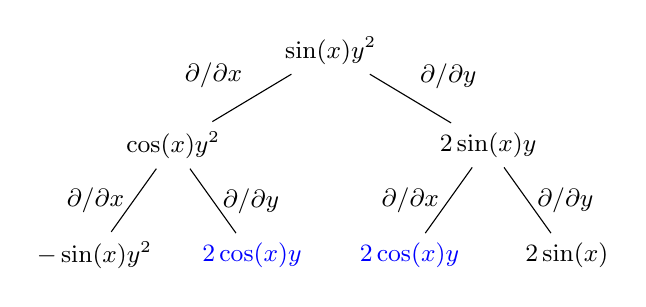
\begin{tikzpicture}[every node/.style={font=\small}]
\node (f) at (0,0) {$\sin(x)y^2$};
\node (x) at (-2,-1.2) {$\cos(x)y^2$};
\node (y) at (2,-1.2) {$2\sin(x)y$};
\node (xx) at (-3,-2.6) {$-\sin(x)y^2$};
\node[blue] (xy) at (-1,-2.6) {$2\cos(x)y$};
\node[blue] (yx) at (1,-2.6) {$2\cos(x)y$};
\node (yy) at (3,-2.6) {$2\sin(x)$};
\draw (f)--node[above left]{$\partial/\partial x$}(x);
\draw (f)--node[above right]{$\partial/\partial y$}(y);
\draw (x)--node[left]{$\partial/\partial x$}(xx);
\draw (x)--node[right]{$\partial/\partial y$}(xy);
\draw (y)--node[left]{$\partial/\partial x$}(yx);
\draw (y)--node[right]{$\partial/\partial y$}(yy);
\end{tikzpicture}
\end{center}
\end{frame}
% Diapositiva original 38
\begin{frame}{Teorema de Schwarz}
\textbf{Ejercicio}\par Determinar si se cumple el teorema de Schwarz para\[f(x,y)=e^{x^2+y^2}.\]
\end{frame}
% Diapositiva original 39
\begin{frame}{Matriz hessiana}
\small Dada una función real $f$ de $n$ variables reales, si todas sus segundas derivadas parciales existen, la matriz hessiana $H_f$ es cuadrada, de tamaño $n$. El elemento de la fila $i$, columna $j$, es $\partial^2f/(\partial x_i\partial x_j)$.
\[H_f=\begin{pmatrix}
\frac{\partial^2f}{\partial x_1^2}&\frac{\partial^2f}{\partial x_1\partial x_2}&\cdots&\frac{\partial^2f}{\partial x_1\partial x_n}\\
\frac{\partial^2f}{\partial x_2\partial x_1}&\frac{\partial^2f}{\partial x_2^2}&\cdots&\frac{\partial^2f}{\partial x_2\partial x_n}\\
\vdots&\vdots&\ddots&\vdots\\
\frac{\partial^2f}{\partial x_n\partial x_1}&\frac{\partial^2f}{\partial x_n\partial x_2}&\cdots&\frac{\partial^2f}{\partial x_n^2}
\end{pmatrix}.\]
\end{frame}
% Diapositiva original 40
\begin{frame}{Matriz hessiana}
\textbf{Ejemplo}\par Calcular la matriz hessiana de\[f(x,y)=e^{x^2+y^3}.\]
\end{frame}
% Diapositiva original 41
\begin{frame}{Matriz hessiana}
\small\textbf{Ejemplo}\[f(x,y)=e^{x^2+y^3}\]
\[f_x=2xe^{x^2+y^3},\qquad f_y=3y^2e^{x^2+y^3}.\]
\[\begin{aligned}
f_{xx}&=(2+4x^2)e^{x^2+y^3},\\
f_{xy}&=6xy^2e^{x^2+y^3}=f_{yx},\\
f_{yy}&=(6y+9y^4)e^{x^2+y^3}.
\end{aligned}\]
\end{frame}
% Diapositiva original 42
\begin{frame}{Matriz hessiana}
\textbf{Ejemplo}\par Calcular la matriz hessiana de
\[f(x,y)=e^{x^2+y^3}.\]
\[H_f=\begin{pmatrix}
(2+4x^2)e^{x^2+y^3}&6xy^2e^{x^2+y^3}\\
6xy^2e^{x^2+y^3}&(6y+9y^4)e^{x^2+y^3}
\end{pmatrix}.\]
\end{frame}
% Diapositiva original 43
\begin{frame}{Punto mínimo y valor mínimo}
Dada una función $f(x,y)$ y un punto $(a,b)$ de su dominio $D$, se dice que $(a,b)$ es un punto mínimo absoluto si
\[f(a,b)\le f(x,y)\qquad\text{para todo }(x,y)\in D.\]
Si la desigualdad se verifica para todos los puntos del dominio que pertenecen a un disco centrado en $(a,b)$, se dice que $(a,b)$ es un punto mínimo relativo o local.
\end{frame}
% Diapositiva original 44
\begin{frame}{Extremos relativos: mínimos}
\figura{minimos.png}{.95}{.80}
\end{frame}
% Diapositiva original 45
\begin{frame}{Punto máximo y valor máximo}
Dada una función $f(x,y)$ y un punto $(a,b)$ de su dominio $D$, se dice que $(a,b)$ es un punto máximo absoluto si
\[f(a,b)\ge f(x,y)\qquad\text{para todo }(x,y)\in D.\]
Si la desigualdad se verifica para todos los puntos del dominio que pertenecen a un disco centrado en $(a,b)$, se dice que $(a,b)$ es un punto máximo relativo o local.
\end{frame}
% Diapositiva original 46
\begin{frame}{Extremos relativos: máximos}
\figura{maximos.png}{.95}{.80}
\end{frame}
% Diapositiva original 47
\begin{frame}{Puntos y valores extremos}
Los puntos del dominio de la función que son mínimos o máximos relativos se llaman puntos extremos. Los valores de la función en estos puntos se llaman valores extremos.
\end{frame}
% Diapositiva original 48
\begin{frame}{Punto crítico}
Un punto $(a,b)$ se llama punto crítico de $f(x,y)$ si:
\begin{enumerate}
\item $(a,b)\in D$.
\item $f_x(a,b)=0$ y $f_y(a,b)=0$.
\end{enumerate}
También se consideran críticos los puntos interiores del dominio donde alguna de las derivadas parciales no existe.
\end{frame}
% Diapositiva original 49
\begin{frame}{Condición necesaria de extremo}
Si una función de dos variables $f$ tiene un extremo local en un punto interior $(a,b)$ y sus derivadas parciales existen allí, entonces
\[\nabla f(a,b)=\mathbf0;\qquad f_x(a,b)=0,\quad f_y(a,b)=0.\]
Como consecuencia, $(a,b)$ es un punto crítico de $f$.
\end{frame}
% Diapositiva original 50
\begin{frame}{Puntos de silla}
\figura{silla.png}{.95}{.40}
\small En la figura, $a$, $b$ y $c$ son puntos críticos: el gradiente se anula en cada uno. $a$ y $b$ son extremos relativos, pero $c$ no lo es. $c$ se llama punto de silla o de ensilladura.
\medskip

Un punto crítico puede ser un extremo relativo o, si hay valores mayores y menores arbitrariamente cerca de él, un punto de silla.
\end{frame}
% Diapositiva original 51
\begin{frame}{Clasificación de puntos críticos}
En funciones de dos variables, los puntos críticos pueden ser máximos, mínimos o puntos de silla.
\medskip

¿Cómo determinar de qué tipo es cada uno?
\medskip

Con el criterio de las segundas derivadas o de la matriz hessiana, cuando éste permite decidir.
\end{frame}
% Diapositiva original 52
\begin{frame}{Procedimiento para determinar extremos}
\figura{procedimiento.png}{.95}{.81}
\end{frame}
% Diapositiva original 53
\begin{frame}{Criterio de las segundas derivadas}
\small Sea $f$ con segundas derivadas parciales continuas cerca de $(a,b)$, y con $f_x(a,b)=f_y(a,b)=0$.
\[G=\det H_f(a,b)=f_{xx}(a,b)f_{yy}(a,b)-[f_{xy}(a,b)]^2.\]
\begin{itemize}
\item Mínimo local si $G>0$ y $f_{xx}(a,b)>0$.
\item Máximo local si $G>0$ y $f_{xx}(a,b)<0$.
\item Punto de silla si $G<0$.
\end{itemize}
Si $G=0$, el criterio no permite decidir.
\end{frame}
% Diapositiva original 54
\begin{frame}{Criterio de los valores propios}
\small Sea $f$ con segundas derivadas parciales continuas cerca de $(a,b)$ y con gradiente nulo en ese punto. Los valores propios de su hessiana se calculan mediante
\[\det\bigl(H_f(a,b)-\lambda I\bigr)=0.\]
\begin{enumerate}
\item Mínimo relativo: todos los valores propios son positivos.
\item Máximo relativo: todos los valores propios son negativos.
\item Punto de silla: hay valores propios positivos y negativos.
\end{enumerate}
Si alguno es cero, el criterio puede no decidir. Si ya hay valores propios de ambos signos, sí se concluye que es un punto de silla.
\end{frame}
% Diapositiva original 55
\begin{frame}{Clasificación de puntos críticos}
\textbf{Ejemplo}\par Determinar los máximos, mínimos o puntos de ensilladura de\[f(x,y)=xy-2x-y.\]
\end{frame}
% Diapositiva original 56
\begin{frame}{Clasificación de puntos críticos}
\textbf{Ejemplo}\par Determinar los máximos, mínimos o puntos de ensilladura de\[f(x,y)=xy-2x-y.\]\textbf{1)} Calculamos las derivadas parciales y las igualamos a cero:
\[f_x=y-2,\qquad f_y=x-1.\]
\[y-2=0\Rightarrow y=2,\qquad x-1=0\Rightarrow x=1.\]
\end{frame}
% Diapositiva original 57
\begin{frame}{Clasificación de puntos críticos}
\small\textbf{Ejemplo}\par Determinar los máximos, mínimos o puntos de ensilladura de\[f(x,y)=xy-2x-y.\]\textbf{1)} Calculamos las derivadas parciales y las igualamos a cero:
\[f_x=y-2,\qquad f_y=x-1.\]
\[y-2=0\Rightarrow y=2,\qquad x-1=0\Rightarrow x=1.\]\textbf{2)} Calculamos las derivadas parciales segundas:
\[f_{xx}=0,\quad f_{yy}=0,\quad f_{xy}=f_{yx}=1.\]
\textbf{3)} Calculamos el determinante de la hessiana:
\[G=f_{xx}f_{yy}-f_{xy}f_{yx}=-1<0.\]
\end{frame}
% Diapositiva original 58
\begin{frame}{Clasificación de puntos críticos}
\small\textbf{Ejemplo}\par\[G=\det H_f(a,b)=f_{xx}(a,b)f_{yy}(a,b)-[f_{xy}(a,b)]^2.\]
\begin{itemize}
\item Mínimo local si $G>0$ y $f_{xx}(a,b)>0$.
\item Máximo local si $G>0$ y $f_{xx}(a,b)<0$.
\item Punto de silla si $G<0$.
\end{itemize}
Si $G=0$, el criterio no permite decidir.\medskip En este ejemplo, $G=-1<0$. Por tanto, $(1,2)$ es un punto de silla.
\end{frame}
% Diapositiva original 59
\begin{frame}{Clasificación de puntos críticos}
\textbf{Ejemplo}\par Determinar los máximos, mínimos o puntos de ensilladura de\[f(x,y)=e^{4y-y^2-x^2}.\]
\end{frame}
% Diapositiva original 60
\begin{frame}{Clasificación de puntos críticos}
\small\textbf{Ejemplo}\par Determinar los máximos, mínimos o puntos de ensilladura de\[f(x,y)=e^{4y-y^2-x^2}.\]Calculamos las derivadas parciales y las igualamos a cero:
\[f_x=-2xe^{4y-y^2-x^2},\qquad f_y=(4-2y)e^{4y-y^2-x^2}.\]
\[-2xe^{4y-y^2-x^2}=0,\qquad(4-2y)e^{4y-y^2-x^2}=0.\]
\[x=0,\qquad y=2\qquad\Longrightarrow\qquad(0,2).\]
\end{frame}
% Diapositiva original 61
\begin{frame}{Clasificación de puntos críticos}
\small\textbf{Ejemplo}\par Determinar los máximos, mínimos o puntos de ensilladura de\[f(x,y)=e^{4y-y^2-x^2}.\]Calculamos las derivadas parciales segundas:
\[\begin{aligned}
f_{xx}&=(-2+4x^2)e^{4y-y^2-x^2},&f_{xx}(0,2)&=-2e^4,\\
f_{yy}&=\bigl[-2+(4-2y)^2\bigr]e^{4y-y^2-x^2},&f_{yy}(0,2)&=-2e^4,\\
f_{xy}&=-2x(4-2y)e^{4y-y^2-x^2}=f_{yx},&f_{xy}(0,2)&=0.
\end{aligned}\]
\end{frame}
% Diapositiva original 62
\begin{frame}{Clasificación de puntos críticos}
\small\textbf{Ejemplo}\par\[G=\det H_f(a,b)=f_{xx}(a,b)f_{yy}(a,b)-[f_{xy}(a,b)]^2.\]
\begin{itemize}
\item Mínimo local si $G>0$ y $f_{xx}(a,b)>0$.
\item Máximo local si $G>0$ y $f_{xx}(a,b)<0$.
\item Punto de silla si $G<0$.
\end{itemize}
Si $G=0$, el criterio no permite decidir.\medskip En este ejemplo,
\[G=(-2e^4)(-2e^4)-0=4e^8>0,\qquad f_{xx}(0,2)<0.\]
El punto $(0,2)$ es un máximo relativo.
\end{frame}
% Diapositiva original 63
\begin{frame}{Optimización de dos variables}
\textbf{Ejemplo}\par Se decide construir una caja con forma de prisma rectangular y volumen $1000\,\mathrm{cm}^3$. Encontrar sus dimensiones $x,y,z$ de modo que la superficie total de las seis caras sea mínima.
\figura{caja.png}{.65}{.34}
\end{frame}
% Diapositiva original 64
\begin{frame}{Optimización de dos variables}
\small El área total de las seis caras es $A=2xy+2yz+2zx$ y el volumen es $V=xyz=1000$.
\medskip

Despejando $z$ del volumen y sustituyendo en el área:
\[A(x,y)=2xy+2y\frac{1000}{xy}+2x\frac{1000}{xy}=2xy+\frac{2000}x+\frac{2000}y.\]
Es una función de dos variables, con $x,y>0$. Calculamos las primeras derivadas parciales y las igualamos a cero:
\[A_x=2y-\frac{2000}{x^2}=0,\qquad A_y=2x-\frac{2000}{y^2}=0.\]
Resolviendo, $x=y=10$ cm y $z=1000/(xy)=10$ cm.
\end{frame}
% Diapositiva original 65
\begin{frame}{Optimización de dos variables}
\small Calculamos las derivadas parciales segundas:
\[A_{xx}=\frac{4000}{x^3},\qquad A_{yy}=\frac{4000}{y^3},\qquad A_{xy}=A_{yx}=2.\]
Calculamos el determinante de la matriz hessiana en $(10,10)$:
\[G=A_{xx}(10,10)A_{yy}(10,10)-[A_{xy}(10,10)]^2=4\cdot4-2^2=12.\]
Como $G>0$ y $A_{xx}(10,10)>0$, es un mínimo relativo.
\medskip

Con volumen fijo, $2(xy+yz+zx)\ge6(xyz)^{2/3}=600\,\mathrm{cm}^2$. La igualdad se alcanza con $x=y=z=10$ cm: es también el mínimo absoluto.
\end{frame}
% Diapositiva original 66
\begin{frame}{Ejercicios finales}
\small\begin{enumerate}
\item Si $T(x,y)=x^2y+3xy^4$ representa la temperatura en $(x,y)$ y $x=e^t$, $y=\sin t$ son las ecuaciones paramétricas de una curva $C$, calcular la razón de cambio de $T$ a lo largo de la curva.
\item Determinar si se cumple el teorema de Schwarz para $f(x,y)=x^2y^2\sin\!\left(\frac1{xy^2}\right)$ en su dominio.
\item Hallar $f_x$ y $f_y$ para $f(x,y)=\ln\!\left(\frac{x+y}{x-y}\right)$.
\item Encontrar la ecuación del plano tangente a la superficie implícita $3xy+z^2=4$ en $(1,1,1)$.
\end{enumerate}
\end{frame}
% Diapositiva original 67
\begin{frame}{Ejercicios finales}
\small\begin{enumerate}\setcounter{enumi}{4}
\item Dada $f(x,y,z)=2x+3y^2-\sin z$, calcular el vector gradiente.
\item Encontrar el plano tangente al paraboloide $z=\dfrac{x^2+4y^2}{10}$ en $(2,-2,2)$.
\item Determinar la derivada direccional de $f(x,y)=x^2+y^3$ en la dirección del punto $Q(-1,1)$ al punto $R(3,0)$.
\item Calcular la matriz hessiana de $f(x,y)=3xy^2-2y+5x^2y^2$.
\end{enumerate}
\end{frame}
% Diapositiva original 68
\begin{frame}{Ejercicios finales}
\small\begin{enumerate}\setcounter{enumi}{8}
\item Una empresa fabrica y vende dos productos, I y II, que cuestan producir 30 y 20 euros por unidad, respectivamente. Los ingresos por vender $x$ unidades del producto I e $y$ unidades del producto II son
\[98x+112y-0{,}04xy-0{,}1x^2-0{,}2y^2.\]
Encontrar los valores de $x$ e $y$ que maximizan las ganancias de la empresa.
\item Considerar $f(x,y)=xy^2+x^2y+5x-y$. Si estamos en $(1,2)$, ¿en qué dirección decrece más rápidamente la función?
\end{enumerate}
\end{frame}
\end{document}
